%!TEX encoding = UTF-8 Unicode
% $Id: 23-parsing_with_atns.tex 18 2014-03-12 22:35:24Z binghe $

\chapter{使用~ATN 分析句子}
\label{chap:parsing_with_atns}

这一章将介绍这样一种技术,它把非确定性分析器~(parser) \index{parsers,
  nondeterministic 分析器, 非确定性|see{ATNs}} 实现成一种嵌入式的语言。
其中,第一部分将会解释什么是~\textsc{ATN} 分析器,以及它们是如何表示语
法规则的。第二部分会给出一个~\textsc{ATN} 编译器,这个编译器将会使用在
前一章定义的非确定性操作符。最后的几个小节则会展示一个小型
的~\textsc{ATN} 语法,然后看看它在实际中是如何分析一段样本代码的。

\section{背景知识}
\label{sec:background}

扩充转移网络\index{augmented transition networks 扩充转移网
  络|see{ATNs}}~(\textsc{ATN})\index{ATNs},是~Bill Woods\index{Woods,
  William A.} 在~1970 年提出的一种分析器。在那之后,\textsc{ATN} 在自然语
言\index{natural language|see{\textsc{ATN}s}}\index{ATNs!for natural language 用于自然语言}分析领域中作为一种形式
化方法,被广为使用。\note{305} 只消一个小时,你就能写出一个能分析有意义
的英语句子的~\textsc{ATN} 语法。出于这个原因,人们常常在初次见识~\textsc{ATN} 之后,就
会为之着迷。

在~1970 年代,一部分研究者认为~\textsc{ATN} 有朝一日有可能会成为真正感觉有智能的
程序的一部分。尽管时至今日,还持有这一观点的人寥寥可数,不过~ATN 的地位
是不可磨灭的。它虽然没有你分析英语句子那么在行,但是它仍然能分析数量可
观的各种句子。

如果你恪守下面的四个限制条件,\textsc{ATN} 就能大显神通:

\begin{enumerate}
\item 仅限用于语义上有限制的领域,比如说作为某个特定的数据库前端。

\item 不能给它过于困难的输入。比如说,请不要认为它们能像人一样能理解非常
  没有语法的句子。

\item 它们仅仅适用于英语\index{English 英语},或者其他单词的顺序决定其语法结构的语言。比如
  说,\textsc{ATN} 就很可能无法被用来分析那种有屈折变化的语言\footnote{译者
    注:屈折语言~(inflected language),是语言学中的概念,指因为单词的变
    格造成语句本身结构和意思的变化。汉语和英语主要依靠单词的顺序来确定
    其语法结构,而屈折语言则主要根据单词的屈折变化~(inflection) 来表现
    句子中的语法关系,比如说拉丁语和德语。虽然英语不是屈折语言,但是它
    里面还是保留着一些形式的屈折变化。比如我们常见的人称代词的``格''的
    变化,主格的~he 和宾格的~him,属格的~his。它们的词根相同,但是词尾
    的变化导致了词性和意思的变化,但是其在句子中的位置仍是决定其意义的
    主要因素。},如拉丁语\index{Latin}。

\item 不要认为它们总是能正常工作。如果一个应用程序里,只要求它在~90\%的
  情况下正常工作就足够了,那么~\textsc{ATN} 是可以胜任的。倘若要求它不能出丝毫的
  差错,那么就不应该考虑用它。

\end{enumerate}
 
尽管有种种限制,\textsc{ATN} 还是能在很多地方派上用场。最典型的应用案例是用做数
据库的前端。如果你给这种数据库系统配备一个用~\textsc{ATN} 驱动的接口
\index{databases 数据库!natural language interfaces to 的自然语言接
  口},用户查询的时候就不用再构造特定格式的请求,只要用一种形式受限的英
语提问就可以了。

\section{形式化}
\label{sec:the_formalism}

要理解~\textsc{ATN} 的工作机制,我们首先要回忆一下它的全名:扩充转移网络~(Augmented Transition Network)\index{transition networks 转移网络}。所谓转
移网络,是指由有向弧连接起来的一组节点,从根本上可以把它看作一种流程图。
其中一个节点被指定为起始节点,而部分其他节点则被作为终结节点。每条弧上都
带有测试条件,只有对应的条件被满足的时候,状态才能经由这条弧转移到新
的节点。首先,输入是一个序列,并有一个指向当前单词的指针。根据弧进行状
态转移会使指针相应地前进。使用转移网络分析句子的过程,就是找到从起始节
点走到某个终止节点的路径的过程,在这个过程中,所有的转移条件都要满足。

\textsc{ATN} 在这个模型的基础上另加入了两个特性:

\begin{enumerate}

\item \textsc{ATN} 带有寄存器\index{ATNs!registers of 寄存器}。寄存器是有名字的~slot,它可以被用来保存分析过程中
  所需的有关信息。转移弧除了能进行条件判断之外,还会设置和修改寄存器中
  的内容。

\item \textsc{ATN} 的结构可以是递归的\index{ATNs!recursion in 递归}。转移弧可以这样要求:如果要通过这条弧,分
  析过程必须能通过某个子网络。

\end{enumerate}

而终结节点则使用寄存器中累积得到信息来建立列表结构并返回它,这种返回结
果的方式和函数返回值的方式非常像。实际上,除了它具有的非确定性之
外,\textsc{ATN} 的行为方式和函数式编程语言很相似。

图~\ref{fig:a_very_small_atn} 中定义的~\textsc{ATN} 几乎是最简单的~\textsc{ATN} 了。它
能分析形如``Spot runs''~(``电视广告插播中'') 的名词 -- 动词型句子。这
种~\textsc{ATN} 的网络表示如图~\ref{fig:graph_of_a_small_atn} 所示。

\begin{figure}
\begin{lstlisting}
(defnode s
  (cat noun s2
    (setr subj *)))

(defnode s2
  (cat verb s3
    (setr v *)))

(defnode s3
  (up '(sentence
         (subject ,(getr subj))
         (verb ,(getr v)))))
\end{lstlisting}
  \caption{一个微型~ATN}
  \label{fig:a_very_small_atn}
\end{figure}

\begin{figure}
\begin{center}
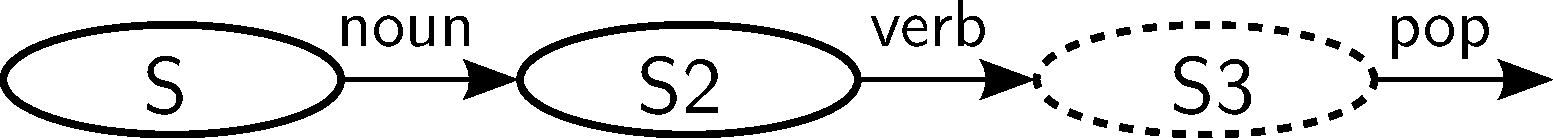
\includegraphics[width=.5\textwidth]{mini-atn.pdf}
\end{center}
  \caption{微型~ATN 的图示}
  \label{fig:graph_of_a_small_atn}
\end{figure}

当~\textsc{ATN} 分析输入序列~\texttt{(spot runs)} 时,它是如何工作的呢?第一个节
点有一条出弧~(outgoing arc),或者说一条类型弧~(cat),这条弧指向节
点~\texttt{s2}。这事实上是表示:如果当前单词是个名词的话,你就可以通过
我;如果你通过我的话,你必须把当前单词~(即~\texttt{*}) 保存
在~\texttt{subj} 寄存器中。因而,当离开这个节点时,
\verb|subj| 的内容就变成了~\verb|spot|。

总是有个指针指向当前的单词。在开始的时候,它指向句子的第一个单
词。在经过~cat 弧的时候,指针会往前移动一个单词。因此,在我们到
达~\texttt{s2} 节点的时候,当前节点会变成第二个单词,即~\texttt{runs}。
第二条弧线和第一条一样,不同之处在于它要求的是个动词。它发现
了~\texttt{runs},并把它保存在寄存器~\texttt{v} 里面,然后状态就走到
了~\texttt{s3}。

在最后一个节点~\texttt{s3} 上,只有一个~pop 弧~(或称为终止
弧)。(有~pop 弧的节点的外围线是虚线)。由于我们正好在把输入序列读完的时候
通过了~pop 弧,所以我们进行的句子分析是成功的。Pop 弧返回的是一个\bq\index{backquote@backquote (\texttt{`}) \bq!in ATNs}表达
式:

\begin{lstlisting}
(sentence (subject spot)
          (verb runs))
\end{lstlisting}

一个~\textsc{ATN} 是与它所要分析语言的语法相对应的。一个用来分析英语的~\textsc{ATN},如果
规模适中的话,那么它会有一个用来分析句子的主网络,以及用来分析名词短语、
介词短语,以及修饰词组等语法元素的多个子网络。让我们想一想含有介词短语
的名词短语,其中,介词短语也是有可能含有名词短语的,并且这种结构可能
会\emph{无穷无尽}地延续下去。显而易见,要处理下面这种结构的句子,必须
要能支持递归:

\begin{quote} 
  ``the key on the table in the hall of the house on the hill''
\end{quote}

\section{非确定性}
\label{sec:nondeterminism}

尽管我们在这个简单的例子里面没有看出来,但是~\textsc{ATN} 的确是非确定性的。一个
节点可以有多个出弧,而特定的输入可以同时满足一个以上的出弧的条件。举个
例子,一个像样的~\textsc{ATN} 应该既能分析祈使句也能分析陈述句。所以第一个节点要
有向外的~cat 弧,与名词~(用于陈述句) 和动词~(用于祈使句)。

要是句子开头的单词是``time''呢?``time''既是名词又是动词。分析器如何知
道该选哪条弧呢?如果~\textsc{ATN} 是以不确定的方式\index{ATNs!nondeterminism in}运行的,那就意味着用户可以认为
分析器总是会\emph{猜到正确的}那条弧线。如果有弧线会让分析过程走进死胡同,那么它们
是不会被选中的。

实际上,分析器是无法预见未来的。它只是在无路可走,或者读完了输入还没能
结束分析时,通过回溯的方式来表现出老是猜中的表象。不过所有这些回溯的机
制是自动嵌入在~\textsc{ATN} 编译器产生的代码里面的。所以,在编写~\textsc{ATN} 时,我们可
以认为分析器能够猜出来应该选择哪一条弧通过。

就像许多~(也许是绝大多数) 使用非确定性算法的程序所做的那样,\textsc{ATN} 一样,
使用的也是深度优先搜索\index{nondeterministic choice 非确定性选择!depth-first 深度优先!in ATNs@in \textsc{ATN}s}。如果曾有过分析英语的经验,就能很快了解到,任何
句子都有大把的合法分析结果,但是它们中的绝大多数都是没有意义的。在传统
的单处理器电脑上,一样可以迅速得到较好的分析结果。我们不是一下子算出所
有的分析结果,而只是得出最有可能的那个。如果分析结果是合理的,那么我们
就用不着再去搜索其他的分析方式了;否则我们还可以调用~\emph{fail} 继续
搜寻更多其它的方式。

为了控制生成分析结果的先后顺序,程序员需要借助某种办法来控
制~\emph{choose} 尝试各待选项的顺序。深度优先实现并不是唯一一种控制搜
索顺序的办法。除非选择是随机的,否则任意一种实现都会按照其特定的顺序进
行选择。不过,\textsc{ATN} 和~Prolog 一样,深度优先实现是其内化了的实现方式。
在~\textsc{ATN} 中,出弧被选中的顺序就是它们当初被定义的顺序\index{ATNs!order of arcs 转移弧的顺序}。使用这样的设计,程
序员就可以根据优先级来排列转换弧线的定义了。

\section{一个~\textsc{ATN} 编译器}
\label{sec:an_atn_compiler}
\index{embedded languages!ATNs as@\textsc{ATN}s as}
一般来说,一个基于~\textsc{ATN} 的分析器由三个部分组成:\textsc{ATN} 本身、用来遍历这个~\textsc{ATN}
的解释器,还有一个可以用于查询的词典。举个例子,借助词典我们就可以知道
``run''是个动词。说到词典,那是另一个话题了,我们在这里会使用一个比较初
级的手工编制的词典。我们也不用在网络解释器上费心,因为我们会把~\textsc{ATN} 直接
翻译成~Lisp 代码。在这里要介绍的程序被称为~\textsc{ATN} 编译器的原因是,这个程序
能把整个的~\textsc{ATN} 变成对应的代码。节点会成为函数,而转换弧则会变成函数里的
代码块。

第~\ref{chap:functions_as_representation} 章介绍了把函数作为表达方式的用法\index{ATNs!represented as functions 函数作为表达方式}。
这种编程习惯常常能让程序的运行速度更快。在这里,这意味着会免去在运行时
解析网络的开销。而这样处理的缺点在于,如果出了问题的话,分析原因的线索就会更少了,特别
是如果你用的~Common Lisp 实现没有提供~\texttt{function-lambda-expression} 
\footnote{译者注:见~\emph{CLHS} 中 ~\href{http://www.lisp.org/HyperSpec/Body/fun_function-_a-expression.html}{Function
    FUNCTION-LAMBDA-EXPRESSION} 一节。}的时候.

图~\ref{fig:compilation_of_nodes_and_arcs} 中包含了所有用来把~\textsc{ATN} 节点
转换为~Lisp 代码的源程序。其中~\texttt{defnode} 宏被用来定义节点。它本
身生成的代码很有限,就是一个~\texttt{choose},用来在每个转换弧产生的表
达式中进行选择。节点函数有两个参数,分别是~\texttt{pos} 和~\texttt{regs}:
\texttt{pos} 的值是当前的输入指针~(一个整数),而~\texttt{regs} 是当前的
寄存器组~(为一个关联表的列表)。

\begin{figure}
\begin{lstlisting}
(defmacro defnode (name &rest arcs)
  `(=defun ,name (pos regs) (choose ,@arcs)))

(defmacro down (sub next &rest cmds)
  `(=bind (* pos regs) (,sub pos (cons nil regs))
          (,next pos ,(compile-cmds cmds))))

(defmacro cat (cat next &rest cmds)
  `(if (= (length *sent*) pos)
       (fail)
       (let ((* (nth pos *sent*)))
         (if (member ',cat (types *))
             (,next (1+ pos) ,(compile-cmds cmds))
             (fail)))))

(defmacro jump (next &rest cmds)
  `(,next pos ,(compile-cmds cmds)))

(defun compile-cmds (cmds)
  (if (null cmds)
      'regs
      `(,@(car cmds) ,(compile-cmds (cdr cmds)))))

(defmacro up (expr)
  `(let ((* (nth pos *sent*)))
     (=values ,expr pos (cdr regs))))

(defmacro getr (key &optional (regs 'regs))
  `(let ((result (cdr (assoc ',key (car ,regs)))))
     (if (cdr result) result (car result))))

(defmacro set-register (key val regs)
  `(cons (cons (cons ,key ,val) (car ,regs))
	 (cdr ,regs)))

(defmacro setr (key val regs)
  `(set-register ',key (list ,val) ,regs))

(defmacro pushr (key val regs)
  `(set-register ',key
                 (cons ,val (cdr (assoc ',key (car ,regs))))
                 ,regs))
\end{lstlisting}
  \caption{节点和弧的编译}
  \label{fig:compilation_of_nodes_and_arcs}
\end{figure}

宏~\texttt{defnode} 定义了一个宏,这个宏的名字和对应的节点相同。节
点~\texttt{s} 将会被定义成宏~\texttt{s}。这种习惯做法让转换弧知道
如何引用它们的目标节点 \pozhehao{} 它们只要调用和节点同名的宏就可以了。这
同时也意味着,你在给节点取名的时候应该避免和已有的函数或者宏重名,否则
这些函数或宏会被重定义。

调试~\textsc{ATN} 时,需要借助某种~trace\index{ATNs!tracing} 工具。由于节点成为了
函数,所以就用不着自己实现~trace 了。我们可以利用内建的~Lisp 函
数~\verb|trace|\index{trace@\texttt{trace}}。如同第~\pageref{trace} 页
提到的,只要用~\verb|=defun| 定义节点,就意味着我们可以通过告诉~Lisp
\verb|(trace =mods)| 来对节点~\verb|mods| 的分析过程进行~trace。

节点函数体里面的转移弧就是宏调用,而宏调用返回的代码被嵌入
在~\texttt{defnode} 生成的节点函数中。因此,每个节点的出弧都被表示为对
应的代码,分析器每碰到一个节点,都会通过执行~\texttt{choose} 使用非确定
性的机制来对这些代码择一执行。比如下面这个有几条出弧的节点
\begin{lstlisting}
(defnode foo
  <arc 1>
  <arc 2>)
\end{lstlisting}
就会被变换成如下形式的函数定义:
\begin{lstlisting}
(=defun foo (pos regs)
  (choose
    <translation of arc 1>
    <translation of arc 2>))
\end{lstlisting}

\begin{figure}
\begin{lstlisting}
(defnode s
  (down np s/subj
    (setr mood 'decl)
    (setr subj *))
  (cat v v
    (setr mood 'imp)
    (setr subj '(np (pron you)))
    (setr aux nil)
    (setr v *)))
\end{lstlisting}
被宏展开成:
\begin{lstlisting}
(=defun s (pos regs)
  (choose
    (=bind (* pos regs) (np pos (cons nil regs))
      (s/subj pos
              (setr mood 'decl
                    (setr subj * regs))))
    (if (= (length *sent*) pos)
        (fail)
        (let ((* (nth pos *sent*)))
          (if (member 'v (types *))
              (v (1+ pos)
                 (setr mood 'imp
                       (setr subj '(np (pron you))
                             (setr aux nil
                                   (setr v * regs)))))
              (fail))))))
\end{lstlisting}
  \caption{节点函数的宏展开}
  \label{fig:macroexpansion_of_a_node_function}
\end{figure}

图~\ref{fig:macroexpansion_of_a_node_function} 显示了
图~\ref{fig:sentence_network} 中作为~\textsc{ATN} 例子里第一个节点的宏展开前后的
模样。当节点函数~(如~\texttt{s}) 在运行时被调用时,会非确定性地选择一条
转移弧通过。\texttt{pos} 参数将会是在输入句子中的当前位
置,而~\texttt{regs} 则是现有的寄存器数据。

\index{ATNs!arc types 转移弧的种类}
就像在我们最初的那个例子中见到的,cat 弧要求当前的输入单词在语法上属于
某个类型。在~cat 弧的函数体中,符号~\texttt{*} 将会被绑定到当前的输入单
词上。

%% xxx
由~\texttt{down} 定义的~push 弧,则要求对子网络的调用能成功返回。这些弧
函数接受两个目标节点作为参数,它们分别是:子网络目标节
点~\texttt{sub},和当前网络的下个节点,即~\texttt{next}。注意到,虽然
为~cat 弧生成的代码只是调用了网络中的下一个节点,但是为~push 弧生成的代
码使用的是~\texttt{=bind}。在继续转移到~push 弧指向的节点前,程序必须成
功地从子网络返回。 在~\texttt{regs} 被传入子网络前,一组新的空寄存
器~(\texttt{nil})\index{stacks 栈!of ATN registers} 被~cons 到它的前面。在其他类型的转移弧的函数体中,符
号~\texttt{*} 将会被绑定到输入的当前单词上,不过
在~push 弧中,\texttt{*} 则是被绑定到从子网络返回的表达式上。


jump 弧就像发生了短路一样。分析器直接跳到了目标节点,不需要进行条件测
试,同时输入指针没有向前移动。

最后一种转移弧是~pop 弧,这种转移弧由~\texttt{up} 定义。pop 弧是比较不
常见的,原因在于它们没有目标节点。就像~Lisp 的~\texttt{return} 类
似,\texttt{return} 把程序带到的不是一个子函数,而是主调函数,而~pop
弧指向的不是一个新节点,而是把程序带回``调用方''的~push 弧。pop 弧
的~\texttt{=values} ``返回''的是最近的一个~push 弧的~\texttt{=bind}。但
是如第~\ref{sec:the_formalism} 节所述,这产生的结果和一个普通的~Lisp
\texttt{return} 还不一样,\texttt{=bind} 的函数体已经被包在一
个\continuation{}里了,并且被作为参数顺着之后的转移弧一直传下
去,直到~pop 弧的~\texttt{=values} 把``返回''值作为参数调用这个\continuation{}。

第~\ref{chap:nondeterminism} 章描述的两个版本的非确定
性~\emph{choose},分别是:一个快速的~\texttt{choose}
(第~\pageref{fig:scheme_implementation_of_choose_and_fail} 页),虽然它
无法保证在搜索空间里有环的情况下能正常终止;以及一个较慢
的~\texttt{true-choose} (第~\pageref{fig:correct_choose_in_scheme} 页),它
能在有环的情况下仍然正常工作。当然,在一个~\textsc{ATN} 同样有可能存在环,不过只
要在每个环里至少有一个转移弧能推进输入指针,那么分析器迟早都会走到句子
末尾。问题是出在那种不会推进输入指针的那种环上。这里我们有两个方案:
\begin{enumerate}
\item 使用较慢的、真正的非确定性选择操作
  符~(第~\pageref{func:true-choice} 页给出了其深度优先版本)。
\item 使用快速的~\texttt{choose},同时指出:如果定义的网络含有只需要顺
  着~jump 弧就能遍历的环,那么这个定义是错误的\index{ATNs!correctness of 的正确性}。
\end{enumerate}
在图~\ref{fig:compilation_of_nodes_and_arcs} 采用的是第二个方案。

图~\ref{fig:compilation_of_nodes_and_arcs} 中的最后四个定义定义了用来读
取和设置转移弧函数体中寄存器的宏。在这个程序里,寄存器组是用关联表来表
示的。\textsc{ATN} 所使用的并不是寄存器组,而是一系列寄存器组。当分析器进入一个
子网络时,它获得了一组新的空寄存器,这组寄存器被压在了已有寄存器组的上
面。因此,无论何时,所有寄存器构成的集合都是作为一个关联表的列表存在的。

这些预先定义好的寄存器操作符的操作对象都是当前,或者说是最上面的那一组
寄存器: \texttt{getr} 读一个寄存器;\texttt{setr} 设置寄存
器;而~\texttt{pushr} 把一个值加入寄存器。\note{312}
\texttt{setr}\footnote{译者注:原文为~\texttt{getr},根据上下文应
为~\texttt{setr}。}和~\texttt{pushr} 都使用了更基本的寄存器操作
宏:\texttt{set-register}。注意到,寄存器不需要事先声明。不管传
给~\texttt{set-register} 的是什么名字,它都会用这个名字新建一个寄存器。

这些寄存器操作符都是完全非破坏性的。
``Cons,cons,cons'',\texttt{set-register} 念念有词。
这拖慢了操作符运行的速度,同时也产生了大量无用的垃圾。不过,正如
第~\pageref{share-between-continuations} 页解释的,如果程序某一部分构造了一个\continuation{},那
么就不应该破坏性地修改在这个部分用到的对象\index{ATNs!destructive operations in 破坏性的操作}。一个正在运行的线程中的对象
有可能被另一个正被挂起的线程共享。在本例中,在一个分析过程中发现的寄存
器会与许多其他分析过程共享数据结构。如果速度成了问题,我们可以把寄存器
保存在~vector\index{vectors 向量!for ATN registers 用于~ATN 的寄存器} 里面,而不是关联表里,并且把用过的~vector 回收到一个公用
的~vector 池\index{pools 池}中。

push、cat 和~jump 弧都可以包含表达式体。通常情况下,这些表达式只不过会
是一些~\texttt{setr} 罢了。通过对它们的表达式体调
用~\texttt{compile-cmds},这些几类转移弧的展开函数会把一系
列~\texttt{setr} 串在一起,成为一个单独的表达式:
\begin{lstlisting}
> (compile-cmds '((setr a b) (setr c d)))
(SETR A B (SETR C D REGS))
\end{lstlisting}
每个表达式把它后面的那个表达式作为它的最后一个参数安插到自己的参数列表
中,不过最后一个表达式除外,它就是~\texttt{regs}。因此转移弧的函数体中
的一系列表达式就会被转换成一个单独的表达式,这个表达式将会返回新的那些
寄存器。

这个办法让用户能在转移弧的函数体里安插任意的~Lisp 代码,只要把这
些~Lisp 代码用一个~\texttt{progn} 包起来就可以了。举例来说:

\begin{lstlisting}
> (compile-cmds '((setr a b)
                        (progn (princ "ek!"))
                        (setr c d)))
(SETR A B (PROGN (PRINC "ek!") (SETR C D REGS)))
\end{lstlisting}

我们有意让转移弧的函数体中的代码能访问到部分变量。被分析的句子将被放到
全局的~\texttt{*sent*} 里。还有两个词法变量也将是可见的,它们
是:\texttt{pos},它保存着当前的输入指针;以及~\texttt{regs},它被用来
存放当前的所有寄存器。这是又一个有意地利用变量捕捉\index{capture 捕捉!intentional}的实例。如果期望让用
户不能引用这些变量,可以考虑把它们换成\gensym。

宏~\texttt{with-parses} 是在图~\ref{fig:atn:toplevel_macro} 中定义的,它让
我们有个办法能调用~\textsc{ATN}。要调用它,我们应该传给它起始节点的名字、一个需
要分析的表达式,以及一个代码体。这段代码告诉~\texttt{with-parses} 应该
如何处理返回的分析结果。表面上,\texttt{with-parses} 的功能
和~\texttt{dolist} 这种操作符差不多。实际上,在它内部进行的并不是简单的
叠代操作,而是回溯搜索。每次成功的分析动作都会引起
对~\texttt{with-parses} 表达式中的代码体的一次求值。在代码体中,符
号~\texttt{parse} 将会绑定到当前的分析结果上。\texttt{with-parses} 表达
式会返回~\texttt{@},因为这正是~\texttt{fail}在穷途末路时的返回值。

\begin{figure}
\begin{lstlisting}
(defmacro with-parses (node sent &body body)
  (with-gensyms (pos regs)
    `(progn
       (setq *sent* ,sent)
       (setq *paths* nil)
       (=bind (parse ,pos ,regs) (,node 0 '(nil))
         (if (= ,pos (length *sent*))
             (progn ,@body (fail))
             (fail))))))
\end{lstlisting}
  \caption{toplevel 宏}
  \label{fig:atn:toplevel_macro}
\end{figure}

在进一步研究表达能力更强的~\textsc{ATN} 之前,让我们先看一下之前定义的一个微
型~\textsc{ATN} 产生的分析结果。\textsc{ATN} 编译
器~(图~\ref{fig:compilation_of_nodes_and_arcs}) 产生的代码会调
用~\texttt{types},通过它了解单词的在语法上所担当的角色,所以我们需要先
给它下个定义:
\begin{lstlisting}
(defun types (w)
  (cdr (assoc w '((spot noun) (runs verb)))))
\end{lstlisting}

现在我们只要把起始节点作为第一个参数传给~\texttt{with-parses},并调用它:
\begin{lstlisting}
> (with-parses s '(spot runs)
    (format t "Parsing: ~A~%" parse))
Parsing: (SENTENCE (SUBJECT SPOT) (VERB RUNS))
@
\end{lstlisting}

\section{一个~\textsc{ATN} 的例子}
\label{sec:a_sample_atn}

既然我们把~\textsc{ATN} 编译器从头到尾都说清楚了,接下来可以找个例子小试牛刀了。
为了让~\textsc{ATN} 的分析器能处理的句子的类型更多些,你需要把~\textsc{ATN} 网络,而不
是~\textsc{ATN} 编译器弄得更复杂一些。这里展示的编译器之所以还只是个玩具,其原因
是因为它的速度比较慢,而不是它在处理能力上的局限性。

分析器的处理能力~(与处理速度相区别) 源自于它的语法,由于这里篇幅的限
制,所以我们不得不用一个玩具版本来说明问题。从图~\ref{fig:sub-network_for_strings_of_modifiers} 到
图~\ref{fig:sentence_network} 定义了图~\ref{fig:graph_of_a_larger_atn} 中所示的~\textsc{ATN} (或者说一
组~\textsc{ATN})。这个网络的规模正好足够大,使得它能在分析那句经典的分析素
材``Time flies like an arrow''时,能够得出多种分析结果。

\begin{figure}
\begin{center}
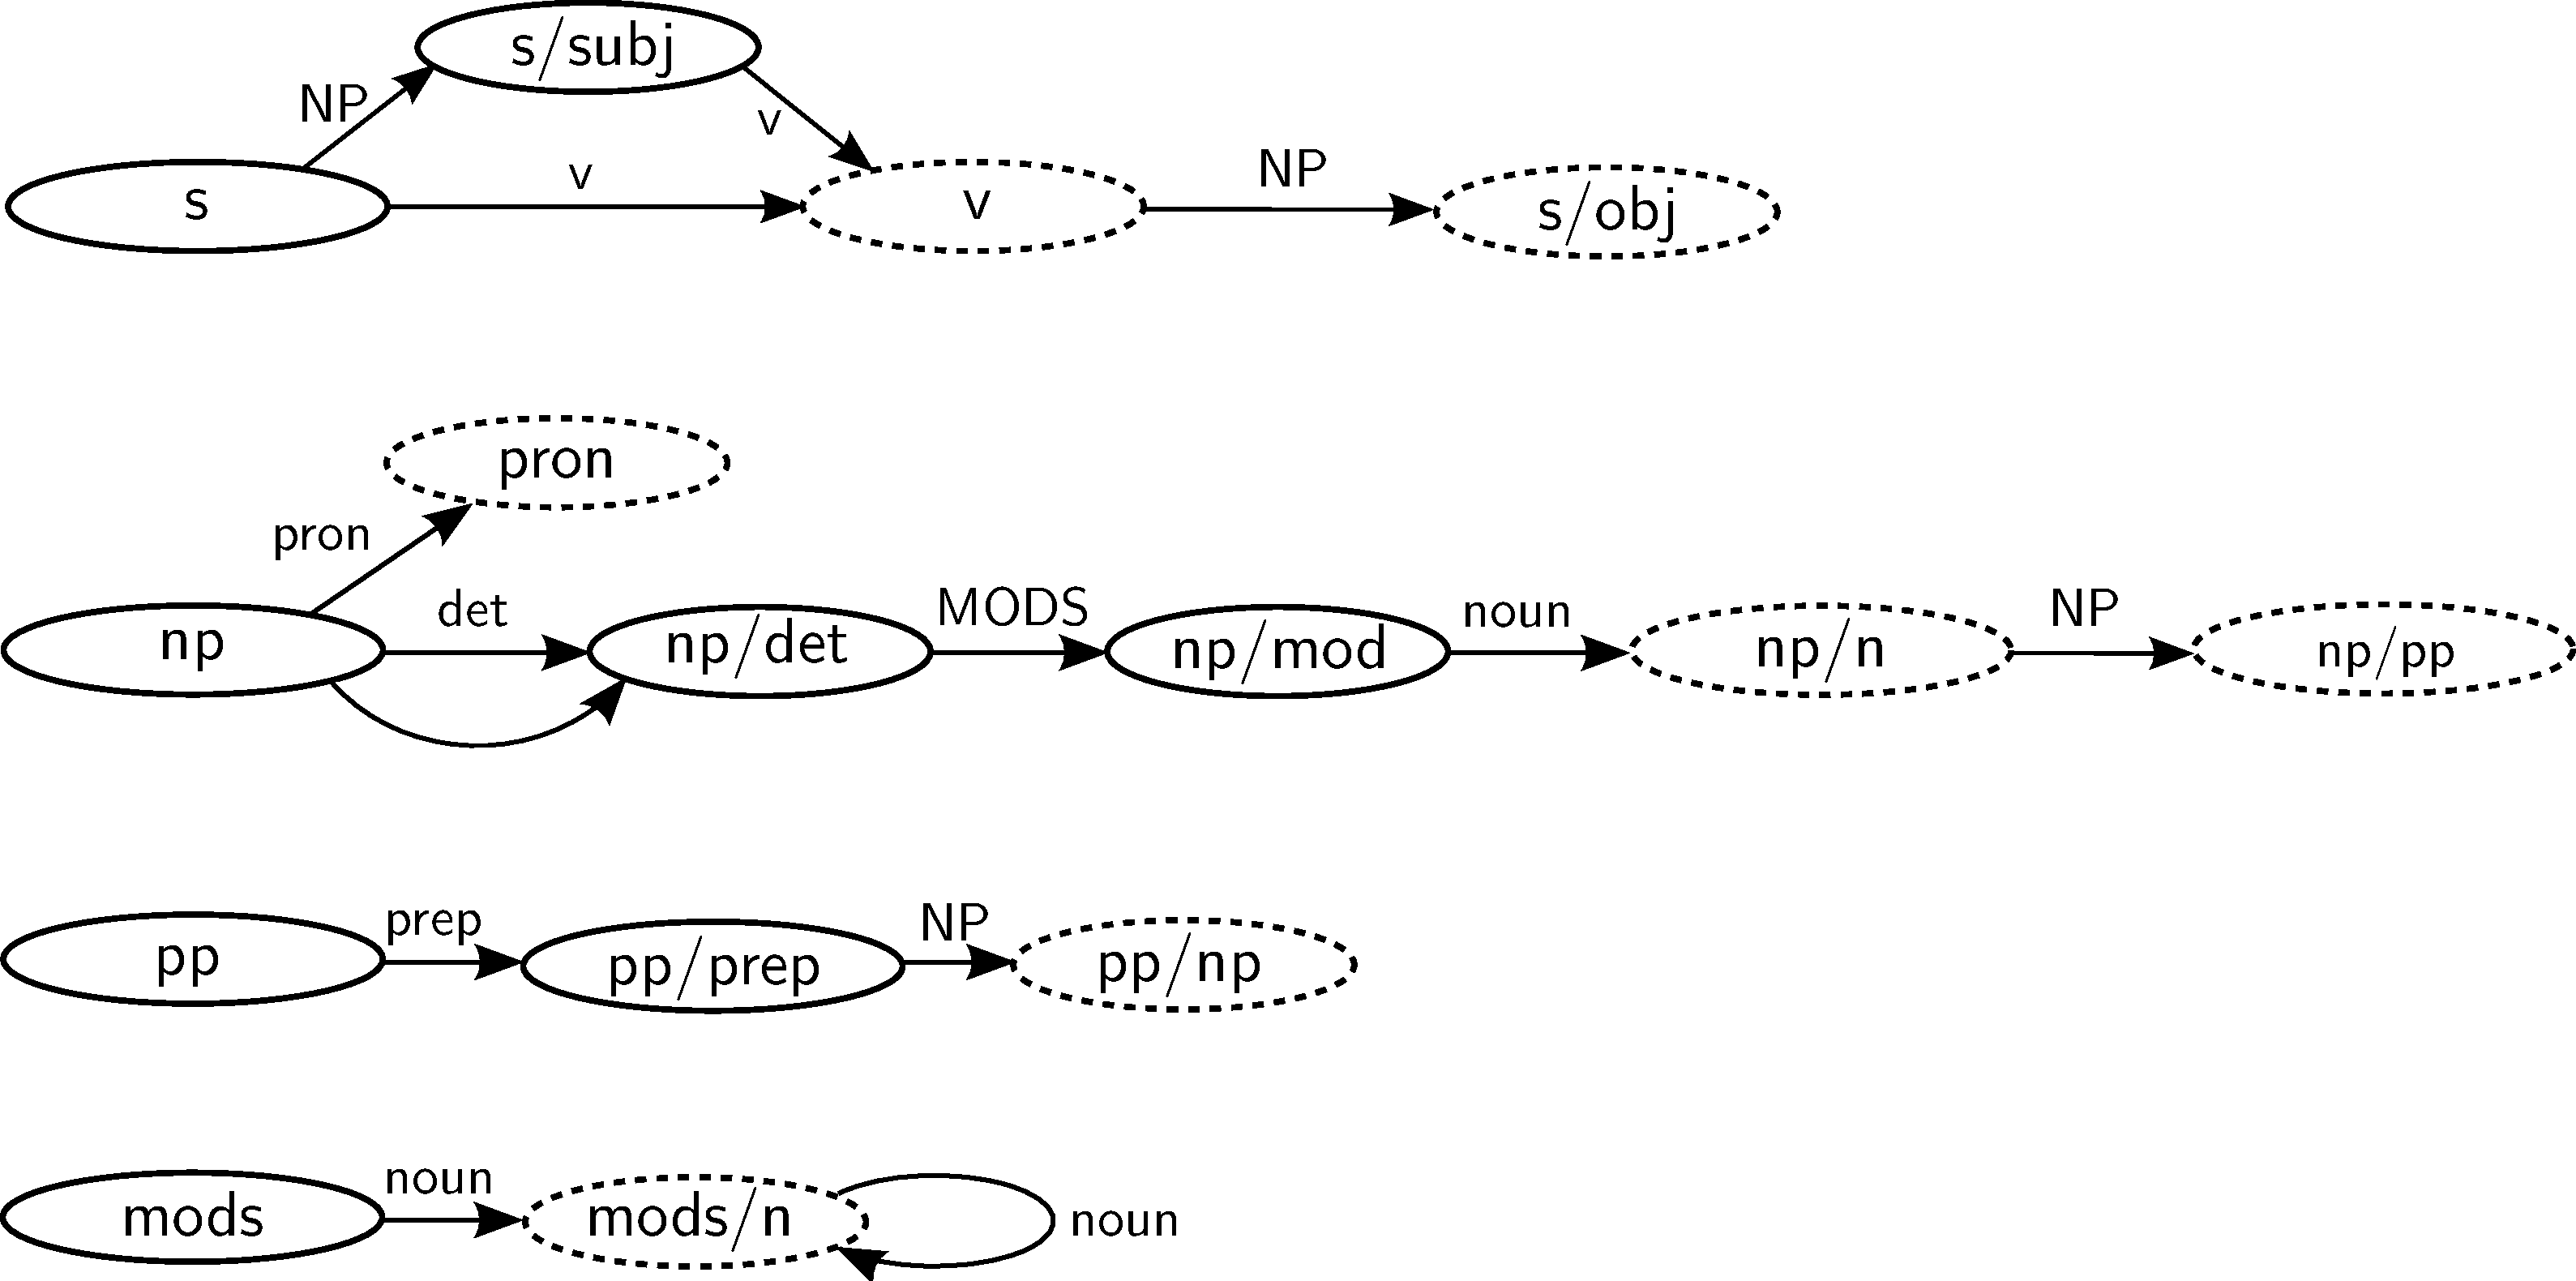
\includegraphics[width=\textwidth]{larger-atn.pdf}
\end{center}
  \caption{一个规模更大的~ATN}
  \label{fig:graph_of_a_larger_atn}
\end{figure}


\begin{figure}
\begin{lstlisting}
(defun types (word)
  (case word
    ((do does did) '(aux v))
    ((time times) '(n v))
    ((fly flies) '(n v))
    ((like) '(v prep))
    ((liked likes) '(v))
    ((a an the) '(det))
    ((arrow arrows) '(n))
    ((i you he she him her it) '(pron))))
\end{lstlisting}
  \caption{象征性的词典}
  \label{fig:nominal_dictionary}
\end{figure}

如果要分析更复杂的输入的话,我们就需要一个稍大的词典。函
数~\texttt{types} (图~\ref{fig:nominal_dictionary}) 提供了一个最基本的词典。它里面定义了
一个由~22 个词组成的词汇库,同时把每个词都和一个列表相关联,列表由一个
或多个单词对应的语法角色构成。


\begin{figure}
\begin{lstlisting}
(defnode mods
  (cat n mods/n
    (setr mods *)))

(defnode mods/n
  (cat n mods/n
    (pushr mods *))
  (up `(n-group ,(getr mods))))
\end{lstlisting}
  \caption{修饰词字符串的子网络}
  \label{fig:sub-network_for_strings_of_modifiers}
\end{figure}

\begin{figure}
\begin{lstlisting}
(defnode np
  (cat det np/det
    (setr det *))
  (jump np/det
    (setr det nil))
  (cat pron pron
    (setr n *)))

(defnode pron
  (up '(np (pronoun ,(getr n)))))

(defnode np/det
  (down mods np/mods
    (setr mods *))
  (jump np/mods
    (setr mods nil)))

(defnode np/mods
  (cat n np/n
    (setr n *)))

(defnode np/n
  (up '(np (det ,(getr det))
           (modifiers ,(getr mods))
           (noun ,(getr n))))
  (down pp np/pp
    (setr pp *)))

(defnode np/pp
  (up '(np (det ,(getr det))
           (modifiers ,(getr mods))
           (noun ,(getr n))
           ,(getr pp))))
\end{lstlisting}
  \caption{名词短语子网络}
  \label{fig:noun_phrase_sub-network}
\end{figure}

\textsc{ATN} 也是由~\textsc{ATN} 本身连接而成的。在本例中,我们的~\textsc{ATN} 部件中最小的一个是
图~\ref{fig:sub-network_for_strings_of_modifiers} 中的~\textsc{ATN}。它分析的是修饰语的字符串,在这里,指的就是名词
的字符串。\texttt{mods} 是第一个节点,它接受一个名词。第二个节点
是~\texttt{mods/n},它会去寻找更多的名词或者返回一个分析结果。

第~\ref{sec:functions_as_properties} 节介绍了把程序写成函数式风格能让程
序更易于测试的缘由:
\begin{enumerate}
\item 在函数式程序中,可以单独地测试程序的组成部件。
\item 在~Lisp 中,可以在~toplevel 的循环里交互地测试函数。
\end{enumerate}

这两条原因合在一起,成为了我们能进行\emph{交互式开发}\index{interactive development}的理由:当我们用~Lisp 写
函数式程序的时候,我们就可以每写一部分代码,就测试它们。

\textsc{ATN} 和函数式程序非常相像\index{ATNs!like functional programs 和函数式程序相像},从它的实现上看,\textsc{ATN} 宏展开\emph{成了}函数式的程序。
这个相似点使得交互式的开发方式也一样适用于~\textsc{ATN} 的开发。我们可以把任意一
个节点作为起点来测试~\textsc{ATN},只要把节点的名字作为~\texttt{with-parses} 的
第一个参数传入:

\begin{lstlisting}
> (with-parses mods '(time arrow)
        (format t "Parsing: ~A~%" parse))
Parsing: (N-GROUP (ARROW TIME))
\end{lstlisting}
接下来的两个网络需要放在一起讨论,因为它们之间是互相递归调用的。
图~\ref{fig:noun_phrase_sub-network} 中定义的网络被用来分析名词短语,它从节点~\texttt{np} 开始。
在图~\ref{fig:prepositional_phrase_sub-network} 中定义的网络则被用来分析介词短语。名词短语有可能含有介
词短语,反之亦然。所以它们两个各自有一个~push 弧,分别调用另一个网络。

名词短语网络中有六个节点。其中,第一个节点~\texttt{np} 有三个选择。如果
它读到了一个代词,那么它就可以转移到节点~\texttt{pron},这会让它弹出这
个网络:
\begin{lstlisting}
> (with-parses np '(it)
    (format t "Parsing: ~A~%" parse))
Parsing: (NP (PRONOUN IT))
@
\end{lstlisting}

另外两个转移弧都指向了节点~\texttt{np/det}:一条弧读入一个限定词~(比如
说~``the''),而另一条弧则直接跳转,不从输入读取任何词。在节
点~\texttt{np/det},两条出弧都通向~\texttt{np/mods};\texttt{np/det} 可
以选择~push 到子网络~\texttt{mods},以此来找出修饰词的字串,或者直
接~jump。节点~\texttt{np/mods} 读入一个名词,然后转移到~\texttt{np/n}。
这个节点要么弹出结果,要么进入介词短语网络,看看能不能碰到个介词短语。
最后的节点,即~\texttt{np/pp},弹出结果。

分析不同类型的名词短语所走过分析路径也各不相同。下面是两个名词短语网络
的分析结果:
\begin{lstlisting}
> (with-parses np '(arrows)
    (pprint parse))
(NP (DET NIL)
    (MODIFIERS NIL)
    (NOUN ARROWS))
@
> (with-parses np '(a time fly like him)
        (pprint parse))
(NP (DET A)
    (MODIFIERS (N-GROUP TIME))
    (NOUN FLY)
    (PP (PREP LIKE)
        (OBJ (NP (PRONOUN HIM)))))
@
\end{lstlisting}

第一次分析在最后~jump 到~\texttt{np/det},再~jump 到~\texttt{np/mods}
读入一个名词,然后~pop 到~\texttt{np/n},从而成功结束。第二次的尝试过程
中没有~jump 过,它首先为了匹配一个修饰词字符串~push 进一个子网络,然后
为了介词短语也进入了一个子网络。这应该是分析器的通病,我们的分析器也不
例外:有些在句法上没有问题的表述在语义上却毫无意义,以致于人都没有办法
看出它们的句法结构。这里,名词短语``a time fly like him''和``a Lisp
hacker like him''的形式就是一样的。

\begin{figure}
\begin{lstlisting}
(defnode pp
  (cat prep pp/prep
    (setr prep *)))
(defnode pp/prep
  (down np pp/np
    (setr op *)))
(defnode pp/np
  (up ‘(pp (prep ,(getr prep))
           (obj ,(getr op)))))
\end{lstlisting}
  \caption{介词短语子网络}
  \label{fig:prepositional_phrase_sub-network}
\end{figure}


\begin{figure}
\begin{lstlisting}
(defnode s
   (down np s/subj
       (setr mood 'decl)
       (setr subj *))
   (cat v v
       (setr mood 'imp)
       (setr subj '(np (pron you)))
       (setr aux nil)
       (setr v *)))

(defnode s/subj
  (cat v v
    (setr aux nil)
    (setr v *)))

(defnode v
  (up `(s (mood ,(getr mood))
          (subj ,(getr subj))
          (vcl (aux ,(getr aux))
               (v ,(getr v)))))
  (down np s/obj
    (setr obj *)))

(defnode s/obj
  (up `(s (mood ,(getr mood))
          (subj ,(getr subj))
          (vcl (aux ,(getr aux))
               (v ,(getr v)))
          (obj ,(getr obj)))))
\end{lstlisting}
  \caption{句子网络}
  \label{fig:sentence_network}
\end{figure}

万事俱备,只欠东风。现在我们缺的就是一个能识别整句结构的网络了。
图~\ref{fig:sentence_network} 中的网络同时能分析祈使句和陈述句。按照习
惯,起始节点被叫做~\texttt{s}。第一个节点首先从一个名词短语开始。第二条
出弧读入一个动词。当句子在句法结构上有歧义时,两条转移弧都可能被满
足,最终得到两个或更多的分析结果,如
图~\ref{fig:two_parsings_for_a_sentence} 所示。第一个分析结果
和``Island nations like a navy''类似,而第二个和``Find someone like a
policeman''是同一种。对于``Time flies like an arrow'',更复杂的~\textsc{ATN} 能找
出六种以上的分析结果。

\begin{figure}
\begin{lstlisting}
> (with-parses s '(time flies like an arrow)
    (pprint parse))
(S (MOOD DECL)
   (SUBJ (NP (DET NIL)
             (MODIFIERS (N-GROUP TIME))
             (NOUN FLIES)))
   (VCL (AUX NIL)
        (V LIKE))
   (OBJ (NP (DET AN)
            (MODIFIERS NIL)
            (NOUN ARROW))))
(MOOD IMP)
   (SUBJ (NP (PRON YOU)))
   (VCL (AUX NIL)
        (V TIME))
   (OBJ (NP (DET NIL)
            (MODIFIERS NIL)
            (NOUN FLIES)
            (PP (PREP LIKE)
                (OBJ (NP (DET AN)
                         (MODIFIERS NIL)
                         (NOUN ARROW)))))))
@
\end{lstlisting}
  \caption{一个句子的两种分析方式}
  \label{fig:two_parsings_for_a_sentence}
\end{figure}

在这一章给出~\textsc{ATN} 编译器的目的更多的在于展示如何提炼出一个~\textsc{ATN} 思路的精
髓,而不是实现一个产品级的软件。如果进行一些很明显的改进,代码的效率就
能显著提升。当速度很重要的时候,用闭包来模拟非确定性这个思路从整体上
说,也许就太慢了。但是如果速度不是关键问题,用本章介绍的这种编程技术可
以写出十分简洁明了的程序。


%%% Local Variables:
%%% coding: utf-8
%%% mode: latex
%%% TeX-master: "onlisp-cn"
%%% End:
